\documentclass[tikz,border=5pt]{standalone}
\usepackage{times}
\usepackage{amsmath,amssymb}
\usetikzlibrary{positioning,fit,arrows.meta,backgrounds,shapes.geometric,calc,shadows,decorations.pathreplacing}

\begin{document}
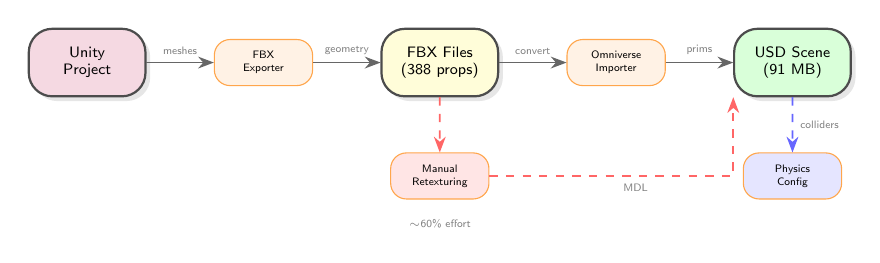
\begin{tikzpicture}[
    scale=0.78,
    transform shape,
    node distance=0.9cm,
    stage/.style={
        draw=black!70,
        rounded corners=3mm,
        minimum width=1.9cm,
        minimum height=1.1cm,
        font=\sffamily\scriptsize,
        fill=white,
        thick,
        align=center,
        drop shadow={opacity=0.2, shadow xshift=0.06cm, shadow yshift=-0.06cm}
    },
    process/.style={
        draw=orange!70,
        fill=orange!10,
        rounded corners=2mm,
        minimum width=1.6cm,
        minimum height=0.75cm,
        font=\sffamily\tiny,
        align=center
    },
    arrow/.style={->, >=Stealth, semithick, color=black!60},
    label/.style={font=\sffamily\tiny, color=black!50}
]

% Source
\node[stage, fill=purple!15] (unity) {Unity\\Project};

% Export stage
\node[process, right=1.1cm of unity] (export) {FBX\\Exporter};

% Intermediate
\node[stage, fill=yellow!15, right=1.1cm of export] (fbx) {FBX Files\\(388 props)};

% Import stage
\node[process, right=1.1cm of fbx] (import) {Omniverse\\Importer};

% Final
\node[stage, fill=green!15, right=1.1cm of import] (usd) {USD Scene\\(91 MB)};

% Arrows
\draw[arrow] (unity) -- node[above, label] {meshes} (export);
\draw[arrow] (export) -- node[above, label] {geometry} (fbx);
\draw[arrow] (fbx) -- node[above, label] {convert} (import);
\draw[arrow] (import) -- node[above, label] {prims} (usd);

% Manual processes below
\node[process, fill=red!10, below=0.9cm of fbx] (retex) {Manual\\Retexturing};
\node[process, fill=blue!10, below=0.9cm of usd] (physics) {Physics\\Config};

% Connect manual processes
\draw[arrow, dashed, red!60] (fbx.south) -- (retex.north);
\draw[arrow, dashed, red!60] (retex.east) -| node[below, label, pos=0.3] {MDL} (usd.south west);
\draw[arrow, dashed, blue!60] (usd.south) -- node[right, label] {colliders} (physics.north);

% Time annotations
\node[font=\sffamily\tiny, color=gray, below=0.2cm of retex] {$\sim$60\% effort};

\end{tikzpicture}
\end{document}
